\documentclass[twoside]{article}
\usepackage{amsgen,amsmath,amstext,amsbsy,amsopn,amssymb,}
\usepackage{graphicx}
\usepackage{epsfig}

\setlength{\oddsidemargin}{0.1 in} \setlength{\evensidemargin}{-0.1
in} \setlength{\topmargin}{-0.6 in} \setlength{\textwidth}{6.5 in}
\setlength{\textheight}{10.4 in} \setlength{\headsep}{0.1 in}
\setlength{\parindent}{0 in} \setlength{\parskip}{0.1 in}

\newcommand{\homework}[2]{
   \pagestyle{myheadings}
   \thispagestyle{plain}
   \newpage
   \setcounter{page}{1}
   \noindent
   \begin{center}
   \framebox{
      \vbox{\vspace{2mm}
       \hbox to 6.28in { {\bf Math 1700:~Elementary Statistics \hfill} }
       \vspace{6mm}
       \hbox to 6.28in { {\Large \hfill #1 (#2)  \hfill} }
       \vspace{6mm}
      \vspace{2mm}}
   }
   \end{center}
   \markboth{#1}{#1}
   \vspace*{4mm}
}

\newcommand{\bbF}{\mathbb{F}}
\newcommand{\bbX}{\mathbb{X}}
\newcommand{\bI}{\mathbf{I}}
\newcommand{\bX}{\mathbf{X}}
\newcommand{\bY}{\mathbf{Y}}
\newcommand{\bepsilon}{\boldsymbol{\epsilon}}
\newcommand{\balpha}{\boldsymbol{\alpha}}
\newcommand{\bbeta}{\boldsymbol{\beta}}
\newcommand{\0}{\mathbf{0}}

\begin{document}

\homework{$3^{th}$ Week Summary}{09/11/25}
\vspace{-.3in}
\begin{itemize}
\item \textbf{Probability}
%\subitem Experiment, Outcome, Sample space, and Event
\subitem An \textbf{experiment} is a process by which a measurement is taken or observations is made
\subitem An \textbf{outcome} is the result of an experiment
\subitem \textbf{Sample space} is a listing of possible outcomes
\subitem An \textbf{event} $A$ is an outcome or a combination of outcomes. 
\item \textbf{Different} type of Probability
\subitem Subjective, Empirical (experimental) and Theoretical
\item \textbf{Tree Diagram}
\item \textbf{Properties} of Probability
\subitem A probability is always a numerical value between zero and one: $0 \leq P(A) \leq 1$
\subitem The sum of probabilities for all \textit{outcomes} of an experiment is equal to exactly one: $\sum_\mathrm{all} P(A) = 1$
\item \textbf{Law of large numbers}: As the number of times an experiment is repeated increases, the ratio of the number of successful occurrences to the number of trials will tend to approach the theoretical probability  of the outcome for an individual trial.
\item \textbf{Odds}: If the odds in favor of an event $A$ are $(a:b)$, then $P(A)=\dfrac{a}{a+b}$
\item \textbf{Conditional probability}: $P(A|B)$ is ``probability of $A$ happening, knowing $B$ has already occurred''
\item \textbf{Rules} of probability 
\subitem Complement Rule: $P(\bar{A})=1-P(A)$
\subitem General Addition Rule: $P(A \ \mathrm{or} \ B) = P(A) + P(B) - P(A \ \mathrm{and} \ B)$
\subitem General Multiplication Rule: $P(A \ \mathrm{and} \ B) = P(A)\cdot P(B|A) = P(B)\cdot P(A|B)$ 
\item \textbf{Mutually exclusive} events: $P(A \ \mathrm{and} \ B) = 0$
\subitem Special Addition Rule: $P(A \ \mathrm{or} \ B \ \mathrm{or} \ C \ \mathrm{or} \ \cdots \ \mathrm{or} \ E) = P(A) + P(B) + P(C) + \cdots + P(E)$
\item \textbf{Independent} events: $P(A) = P(A|B)$, or equivalently: $P(A \ \mathrm{and} \ B) = P(A)\cdot P(B)$
\subitem Special Multiplication Rule: $P(A \ \mathrm{and} \ B \ \mathrm{and} \ C \ \mathrm{and} \ \cdots \ \mathrm{and} \ E) = P(A)\cdot P(B)\cdot P(C)\cdots P(E)$
\begin{figure}[h]
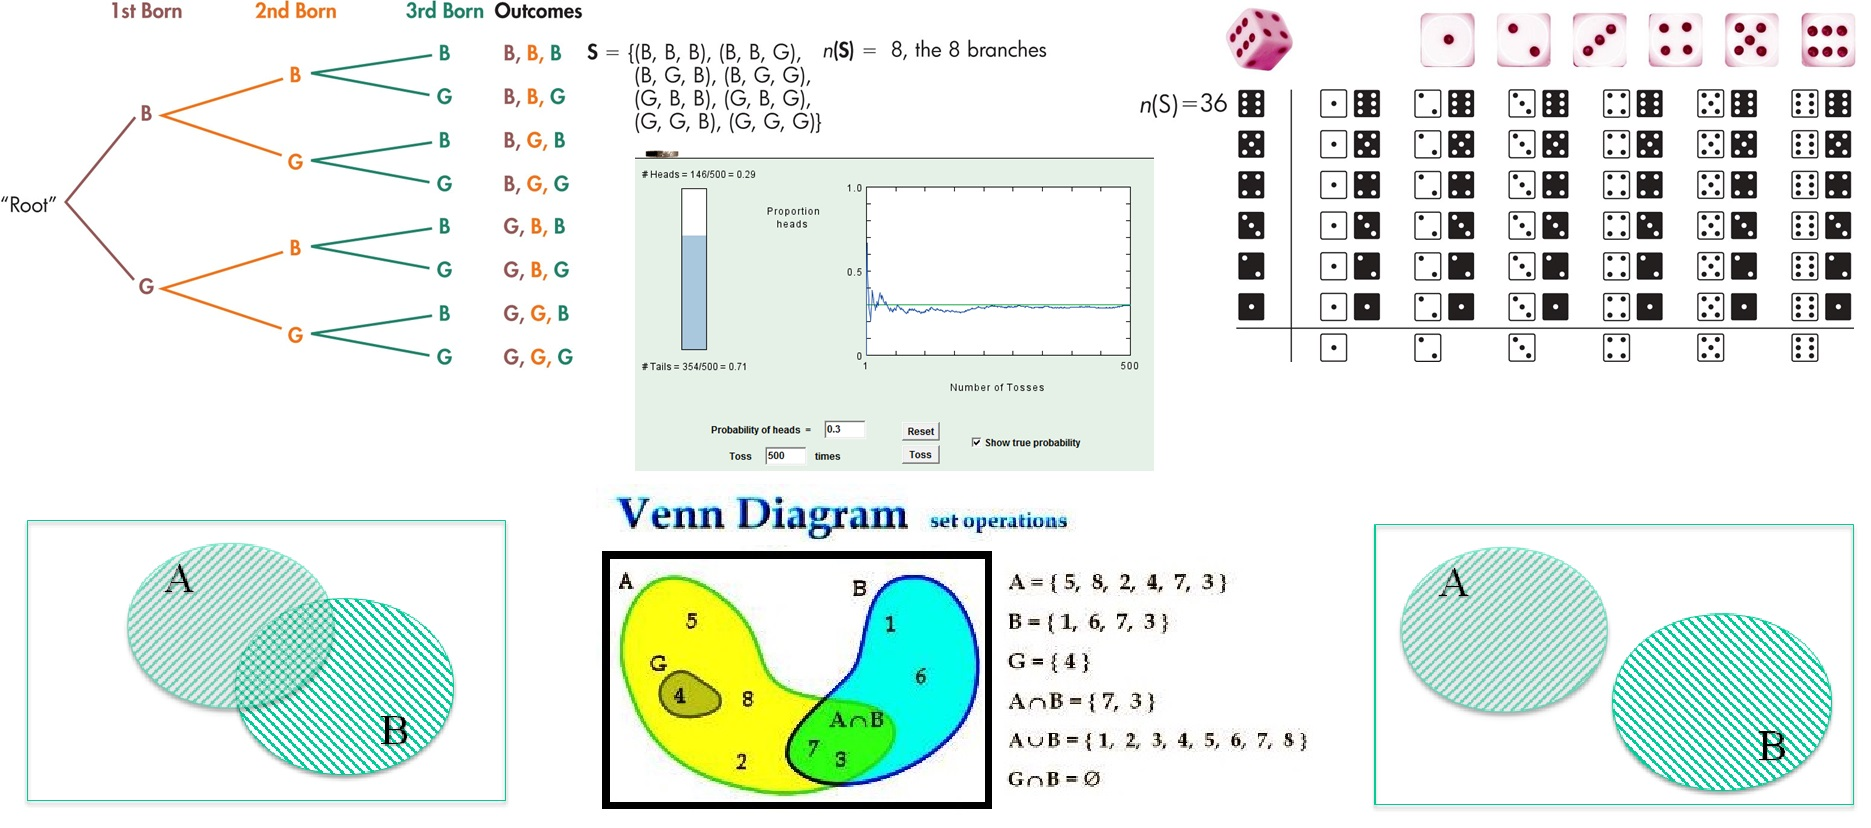
\includegraphics[angle=0,width=\textwidth] {graphs4.jpg}
\end{figure}
\end{itemize}
\end{document}
